\documentclass{beamer}\usepackage[]{graphicx}\usepackage[]{color}
%% maxwidth is the original width if it is less than linewidth
%% otherwise use linewidth (to make sure the graphics do not exceed the margin)
\makeatletter
\def\maxwidth{ %
  \ifdim\Gin@nat@width>\linewidth
    \linewidth
  \else
    \Gin@nat@width
  \fi
}
\makeatother

\definecolor{fgcolor}{rgb}{0.345, 0.345, 0.345}
\newcommand{\hlnum}[1]{\textcolor[rgb]{0.686,0.059,0.569}{#1}}%
\newcommand{\hlstr}[1]{\textcolor[rgb]{0.192,0.494,0.8}{#1}}%
\newcommand{\hlcom}[1]{\textcolor[rgb]{0.678,0.584,0.686}{\textit{#1}}}%
\newcommand{\hlopt}[1]{\textcolor[rgb]{0,0,0}{#1}}%
\newcommand{\hlstd}[1]{\textcolor[rgb]{0.345,0.345,0.345}{#1}}%
\newcommand{\hlkwa}[1]{\textcolor[rgb]{0.161,0.373,0.58}{\textbf{#1}}}%
\newcommand{\hlkwb}[1]{\textcolor[rgb]{0.69,0.353,0.396}{#1}}%
\newcommand{\hlkwc}[1]{\textcolor[rgb]{0.333,0.667,0.333}{#1}}%
\newcommand{\hlkwd}[1]{\textcolor[rgb]{0.737,0.353,0.396}{\textbf{#1}}}%
\let\hlipl\hlkwb

\usepackage{framed}
\makeatletter
\newenvironment{kframe}{%
 \def\at@end@of@kframe{}%
 \ifinner\ifhmode%
  \def\at@end@of@kframe{\end{minipage}}%
  \begin{minipage}{\columnwidth}%
 \fi\fi%
 \def\FrameCommand##1{\hskip\@totalleftmargin \hskip-\fboxsep
 \colorbox{shadecolor}{##1}\hskip-\fboxsep
     % There is no \\@totalrightmargin, so:
     \hskip-\linewidth \hskip-\@totalleftmargin \hskip\columnwidth}%
 \MakeFramed {\advance\hsize-\width
   \@totalleftmargin\z@ \linewidth\hsize
   \@setminipage}}%
 {\par\unskip\endMakeFramed%
 \at@end@of@kframe}
\makeatother

\definecolor{shadecolor}{rgb}{.97, .97, .97}
\definecolor{messagecolor}{rgb}{0, 0, 0}
\definecolor{warningcolor}{rgb}{1, 0, 1}
\definecolor{errorcolor}{rgb}{1, 0, 0}
\newenvironment{knitrout}{}{} % an empty environment to be redefined in TeX

\usepackage{alltt}
\usetheme{default}
%\usetheme{Malmoe}

\title[EC999: Quantitative Text Analysis]{EC999: Classification} \def\newblock{\hskip .11em plus .33em minus .07em}


\def\Tiny{\fontsize{10pt}{10pt}\selectfont}
\def\smaller{\fontsize{8pt}{8pt}\selectfont}

\institute[Warwick]{University of Chicago \& University of Warwick}
\author[Thiemo Fetzer]{Thiemo Fetzer}

 \date{\today}

\usepackage{natbib}
\usepackage{amsmath}
\usepackage{hyperref}
\usepackage{graphicx}
\usepackage{graphics}

\usepackage{amsfonts}
\usepackage{amssymb}
\usepackage{pdfpages}
\usepackage{natbib}
\usepackage{hyperref}
%\usepackage{enumitem}
 \usepackage{pgffor}
\usepackage{booktabs,caption,fixltx2e}
\usepackage[flushleft]{threeparttable}
\usepackage{verbatim} 
\usepackage{cancel}
\newcommand\xxcancel[1]{\xcancel{#1}\vphantom{#1}}

\usepackage{mathtools,xparse}

\newenvironment{Description}
               {\list{}{\labelwidth=0pt \itemindent-\leftmargin
                        \let\makelabel\Descriptionlabel
                        % or whatever
               }}
               {\endlist}
\newcommand*\Descriptionlabel[1]{%
  \hspace\labelsep
  \normalfont%  reset current font setting
  \color{blue}\bfseries\sffamily% or whatever 
  #1}


\setbeamersize{text margin left = 16pt, text margin right = 16pt}
\newcommand{\code}[1]{\texttt{#1}}

\newenvironment<>{algorithm}[1][\undefined]{%
\begin{actionenv}#2%
\ifx#1\undefined%
   \def\insertblocktitle{Algorithm}%
\else%
   \def\insertblocktitle{Algorithm ({\em#1})}%
\fi%
\par%
\mode<presentation>{%
  \setbeamercolor{block title}{fg=white,bg=yellow!50!black}
  \setbeamercolor{block body}{fg=black,bg=yellow!20}
}%
\usebeamertemplate{block begin}\em}
{\par\usebeamertemplate{block end}\end{actionenv}}


\newenvironment<>{assumption}[1][\undefined]{%
\begin{actionenv}#2%
\ifx#1\undefined%
   \def\insertblocktitle{Assumption}%
\else%
   \def\insertblocktitle{Assumption ({\em#1})}%
\fi%
\par%
\mode<presentation>{%
  \setbeamercolor{block title}{fg=white,bg=blue!50!black}
  \setbeamercolor{block body}{fg=black,bg=blue!20}
}%
\usebeamertemplate{block begin}\em}
{\par\usebeamertemplate{block end}\end{actionenv}}



%changing spacing between knitr code and output
\usepackage{etoolbox} 
\makeatletter 
\preto{\@verbatim}{\topsep=0pt \partopsep=0pt } 
\makeatother
\renewenvironment{knitrout}{\setlength{\topsep}{0mm}}{}
\IfFileExists{upquote.sty}{\usepackage{upquote}}{}
\begin{document}



\AtBeginSection[]
{
 \begin{frame}<beamer>
 \frametitle{Plan}
 \tableofcontents[currentsection]
 \end{frame}
}
\maketitle
 

%%%%%%%%%%%%%%%%%%%%%%%%%%%%

%%%%%%%%%%%%%%%%%%%%%%%%%%%%%%%%%%%%%%%%%%%%%%%%%%%%%%%%%%
\begin{frame}{Regression versus Classification}

\begin{itemize}

\item Classification refers to cases where the $y_i$ is a categorical variable, such as Eye color, Gender, Brand, Sentiment = Positive, Negative, Neutral. 

\item Regression refers to cases where the dependent variable is numeric, like price, quantity, ...

\item There are cases, where categorical variables can be given a numeric interpretation, e.g. a categorical variable with two levels can be expressed as a dummy variable/ binary variable, such as Gender = 1 if male, Gender = 0 if female.

\end{itemize}
\end{frame}
%%%%%%%%%%%%%%%%%%%%%%%%%%%%%%%%%%%%%%%%%%%%%%%%%%%%%%%%%%


%%%%%%%%%%%%%%%%%%%%%%%%%%%%%%%%%%%%%%%%%%%%%%%%%%%%%%%%%%
\begin{frame}{Classification Example (1): Land Use Patterns}
  \begin{figure}[h]
\begin{center}
\includegraphics<1>[scale=.5]{figures/landcover-C-plain.png} 
 \includegraphics<2>[scale=.5]{figures/landcover-C.png} 
\end{center}
\caption{\small{Classifiying pixels from satellite imagery into common land use clusters: Cropland, Forest and Shrubland as used in Fetzer and Marden (2016).}}
\end{figure}
\end{frame}
%%%%%%%%%%%%%%%%%%%%%%%%%%%%%%%%%%%%%%%%%%%%%%%%%%%%%%%%%%

%%%%%%%%%%%%%%%%%%%%%%%%%%%%%%%%%%%%%%%%%%%%%%%%%%%%%%%%%%
\begin{frame}{Other Classification Examples}

\begin{enumerate}

\item Fraud detection in financial transaction data

\item News Feed categorization 

\item Email Spam detection

\item Facebook Image Upload Nudity detection

\item Sentiment categorization 

\end{enumerate}

\end{frame}
%%%%%%%%%%%%%%%%%%%%%%%%%%%%%%%%%%%%%%%%%%%%%%%%%%%%%%%%%%

%%%%%%%%%%%%%%%%%%%%%%%%%%%%%%%%%%%%%%%%%%%%%%%%%%%%%%%%%%%%%%%%%%%%%%%%%
\begin{frame}{The General Classification Problem}

\begin{itemize}

\item A qualitative variable takes a value in set $\mathcal{C}$.

\item We will denote $|\mathcal{C}| = c$ the number of different categories.

\item We observe a feature vector $X$ and a responsive variable $Y$ that takes on values from the set $\mathcal{C}$

\item We estimate for each possible value $y \in \mathcal{C}$:

$$ \hat{P}(Y=y|X) $$

\item Following a decision rule, we will assign the ``correct'' label to that category or class $y$, which reduces some form of prediction error.

\item The prediction error we can make here is the share of ``wrongly`` classified categories...

\item How to measure ``wrongly classified'' or ``correct'' label?

\end{itemize}

\end{frame}
%%%%%%%%%%%%%%%%%%%%%%%%%%%%%%%%%%%%%%%%%%%%%%%%%%%%%%%%%%%%%%%%%%%%%%%%%


%%%%%%%%%%%%%%%%%%%%%%%%%%%%%%%%%%%%%%%%%%%%%%%%%%%%%%%%%%
\begin{frame}{Validation Set Approach to Assess Model Accuracy}
  \begin{figure}[h]
\begin{center}
\includegraphics<1>[scale=.35]{figures/validation-set.png} 
\end{center}
\caption{\small{Validation Set Workflow Illustration.}}
\end{figure}
\end{frame}
%%%%%%%%%%%%%%%%%%%%%%%%%%%%%%%%%%%%%%%%%%%%%%%%%%%%%%%%%%

 

\section{Bayes Rule Reminder}

%%%%%%%%%%%%%%%%%%%%%%%%%%%%%%%%%%%%%%%%%%%%%%%%%%%%%%%%%%
\begin{frame}{Bayes Theorem}

\begin{itemize}

\item Bayes Rule States
 $$\underbrace{P(Y|X)}_{posterior} = \frac{\overbrace{P(X|Y)}^{likelihood} \times \overbrace{P(Y)}^{prior}}{\underbrace{P(X)}_{marginal\;likelihood}}$$

\item In case $Y$ and $X$ where independent, $P(Y|X) = P(Y)$, and $P(Y \cap X) = P(Y) P(X)$.

\item $X$ is the evidence, that tells you something about the probability of observing the data $Y$.

\end{itemize}


\end{frame}
%%%%%%%%%%%%%%%%%%%%%%%%%%%%%%%%%%%%%%%%%%%%%%%%%%%%%%%%%%%%%%%%%%%%%%%%%


%%%%%%%%%%%%%%%%%%%%%%%%%%%%%%%%%%%%%%%%%%%%%%%%%%%%%%%%%%
\begin{frame}{Bayes Theorem: Classical Problem}


\begin{quote}
A patient takes a lab test and the result comes back positive. The test returns a correct positive result in only 98\% of the cases in which the disease is actually present, and a correct negative result in only 97\% of the cases in which the disease is not present. You know that 0.008 of the entire population have this disease.
\end{quote}

\end{frame}
%%%%%%%%%%%%%%%%%%%%%%%%%%%%%%%%%%%%%%%%%%%%%%%%%%%%%%%%%%%%%%%%%%%%%%%%%


%%%%%%%%%%%%%%%%%%%%%%%%%%%%%%%%%%%%%%%%%%%%%%%%%%%%%%%%%%
\begin{frame}{Bayes Theorem: Classical Problem}

What are we given? Let $D$ be an indicator if the disaese is present and $+$ indicate whether the test is positive.

\begin{eqnarray*}
P(D) &=& 0.008 \\
P(\neg D) &=& 1-0.008 \\
P(+ | D) &=& 0.98\\
P(- | D) &=& 0.02\\
P(+ | \neg D) &=& 0.03 \\
P(- | \neg D) &=& 0.97
\end{eqnarray*}

What is $P(D | +)$?

$$P(D | +) = \frac{P(D) P(+|C)}{P(+)}$$

\end{frame}
%%%%%%%%%%%%%%%%%%%%%%%%%%%%%%%%%%%%%%%%%%%%%%%%%%%%%%%%%%%%%%%%%%%%%%%%%


%%%%%%%%%%%%%%%%%%%%%%%%%%%%%%%%%%%%%%%%%%%%%%%%%%%%%%%%%%
\begin{frame}{Law of Total Probability}

$$P(D | +) = \frac{P(D) P(+|D)}{P(+)}$$

Using the law of total probability

$$P(+) = P(+|D) P(D) + P(+| \neg D) P(\neg D)$$

$$= 0.98 \times 0.008 + 0.03 \times 0.992 = 0.0376 $$

From this you get:

$$ P(D|+) =  \frac{P(D) P(+|D)}{P(+)}{P(+)} = \frac{ 0.008 \times 0.98}{0.0376} = 0.21$$
\end{frame}
%%%%%%%%%%%%%%%%%%%%%%%%%%%%%%%%%%%%%%%%%%%%%%%%%%%%%%%%%%%%%%%%%%%%%%%%%

\section{Bayesian Decision Theory}

%%%%%%%%%%%%%%%%%%%%%%%%%%%%%%%%%%%%%%%%%%%%%%%%%%%%%%%%%%
\begin{frame}{Prior Information}

\begin{itemize}

\item Suppose you want to categorize some \emph{teaching feedback} into two categories.

\item In our example we have $Y \in \{\text{Positive}, \text{Negative}\}$.

\item Suppose you know what the \emph{priors} are, i.e. you know what the share of positive and negative feedbacks are \emph{in the population}.

\begin{figure}[h]
\begin{center}$
\begin{array}{c}
\includegraphics[scale=.4]<1>{figures/all-feedbacks.png}
\end{array}$
\end{center}
\end{figure}

\end{itemize}


\end{frame}
%%%%%%%%%%%%%%%%%%%%%%%%%%%%%%%%%%%%%%%%%%%%%%%%%%%%%%%%%%%%%%%%%%%%%%%%%

%%%%%%%%%%%%%%%%%%%%%%%%%%%%%%%%%%%%%%%%%%%%%%%%%%%%%%%%%%
\begin{frame}{Best Decision Without Additional Information}

\begin{itemize}

\item Suppose you now receive a new feedback $\tilde{Y}$, and you want to categorize it \emph{without any additional information}

\item What decision / assignment rule would minimize the missclassification error?

\end{itemize}

Clearly this should be

$$ \tilde{Y} = \begin{cases} +  &\mbox{if } P(+) > P(-)  \\ 
 - & \mbox{if } P(+) < P(-)  \end{cases}   $$

What is the error that we make with this \emph{decision rule}?

$$P(error) = \min\{P(+), P(-) \}$$

So here, we would assign any feedback coming in as negative $-$; the maximum error we can make is 18\%.
\end{frame}
%%%%%%%%%%%%%%%%%%%%%%%%%%%%%%%%%%%%%%%%%%%%%%%%%%%%%%%%%%%%%%%%%%%%%%%%%



%%%%%%%%%%%%%%%%%%%%%%%%%%%%%%%%%%%%%%%%%%%%%%%%%%%%%%%%%%
\begin{frame}{Best Decision With Additional Information}

\begin{itemize}

\item Suppose you now have additional information $X$, let that information be the number of characters contained in a feedback. 

\item Suppose that the distribution of the number of characters is smooth in the population. 

\item Plot the density function $p(x|+)$ and $p(x|-)$.

\end{itemize}

\begin{figure}[h]
\begin{center}$
\begin{array}{c}
\includegraphics[scale=.4]<1>{figures/class-conditionals.png}
\end{array}$
\end{center}
\end{figure}

\end{frame}
%%%%%%%%%%%%%%%%%%%%%%%%%%%%%%%%%%%%%%%%%%%%%%%%%%%%%%%%%%%%%%%%%%%%%%%%%


%%%%%%%%%%%%%%%%%%%%%%%%%%%%%%%%%%%%%%%%%%%%%%%%%%%%%%%%%%
\begin{frame}{Using Bayes Rule}

\begin{itemize}

\item For every value of $x$, we can compute the \emph{posterior} probability using Bayes rule.

 $$\underbrace{P(+|x)}_{posterior} = \frac{\overbrace{p(x|+)}^{likelihood} \times \overbrace{P(+)}^{prior}}{\underbrace{p(x)}_{marginal\;likelihood}}$$

where $$p(x) = p(x|+) P(+) + p(x|-) P(-)$$

\end{itemize}
 
\end{frame}
%%%%%%%%%%%%%%%%%%%%%%%%%%%%%%%%%%%%%%%%%%%%%%%%%%%%%%%%%%%%%%%%%%%%%%%%%


%%%%%%%%%%%%%%%%%%%%%%%%%%%%%%%%%%%%%%%%%%%%%%%%%%%%%%%%%%
\begin{frame}{Using Bayes Rule}

\begin{itemize}

\item Plot the posterior densities $p(+|x)$ and $p(-|x)$.

\begin{figure}[h]
\begin{center}$
\begin{array}{c}
\includegraphics[scale=.4]<1>{figures/posteriors.png}
\end{array}$
\end{center}
\end{figure}

\item How would you now decide on which label to assign? I.e. what is the decision rule that minimzes test error?

\end{itemize}
 
\end{frame}
%%%%%%%%%%%%%%%%%%%%%%%%%%%%%%%%%%%%%%%%%%%%%%%%%%%%%%%%%%%%%%%%%%%%%%%%%



%%%%%%%%%%%%%%%%%%%%%%%%%%%%%%%%%%%%%%%%%%%%%%%%%%%%%%%%%%
\begin{frame}{MAP Decision Rule}

\begin{itemize}

\item It seems intuitive, that you should assign 

$$ \tilde{Y} = \begin{cases} +  &\mbox{if } P(+|x) > P(-|x)  \\ 
 - & \mbox{if } P(+|x) < P(-|x)  \end{cases}   $$

\item This is called the \textbf{Maximum A Posteriori} decision rule.

$$P(+|x) >  P(-|x) $$

\item This boils down to (after plugging in)
$$\frac{p(x|+) \times P(+)}{p(x)} > \frac{p(x|-) \times P(-)}{p(x)}$$

$$\frac{p(x|+)}{p(x|-)} > \frac{P(-)}{P(+)}$$

\item Here, we have just two values that $Y$ can take, so the decision rule is
$$P(+|x) > P(-|x) \Rightarrow  P(+|x) > 1-  P(+|x) \Rightarrow  P(+|x) > 1/2$$

\end{itemize}
 
\end{frame}
%%%%%%%%%%%%%%%%%%%%%%%%%%%%%%%%%%%%%%%%%%%%%%%%%%%%%%%%%%%%%%%%%%%%%%%%%


%%%%%%%%%%%%%%%%%%%%%%%%%%%%%%%%%%%%%%%%%%%%%%%%%%%%%%%%%%
\begin{frame}{MAP Decision Rule Minimizes Test Error}

\begin{itemize}

\item It turns out that the MAP decision rule is \emph{Bayes optimal}, it minimizes overall test error. We do not provide a formal proof, but the intuition is given

\item What is the error that we make incorporating the information contained in $x$?

$$P(error|x) = \min\{P(+|x), P(-|x) \}$$

\item The total error over all $x$ would be: 

$$ P(error) = \int_{0}^{\infty} \overbrace{p(error, x)}^{\text{joint}} dx = \int_{0}^{\infty} P(error|x) p(x) dx$$

\item  MAP decision rule minimizes this error, because for every value of $x$, we choose

$$\min\{P(+|x), P(-|x) \}$$

\end{itemize}
 
\end{frame}
%%%%%%%%%%%%%%%%%%%%%%%%%%%%%%%%%%%%%%%%%%%%%%%%%%%%%%%%%%%%%%%%%%%%%%%%%


\section{Classification Error}

%%%%%%%%%%%%%%%%%%%%%%%%%%%%%%%%%%%%%%%%%%%%%%%%%%%%%%%%%%
\begin{frame}{Classification - Types of Errors}

\begin{itemize}

\item In regression, we would evaluate the performance of a predictive model $\hat{f}$ by studying \emph{MSE} on a validation set.

$$ MSE = \frac{1}{n} \sum_{j}^{n} (y_j - \hat{f(x_{ij})})^2$$

\item For numeric variables, we can over-estimate or underestimate. We can tweak our objective function used to estimate the coefficients to penalize over- versus underestimates.


\end{itemize}
 
\end{frame}
%%%%%%%%%%%%%%%%%%%%%%%%%%%%%%%%%%%%%%%%%%%%%%%%%%%%%%%%%%%%%%%%%%%%%%%%%


%%%%%%%%%%%%%%%%%%%%%%%%%%%%%%%%%%%%%%%%%%%%%%%%%%%%%%%%%%
\begin{frame}[fragile]{Test and Training Error}

\begin{itemize}

\item We have argued that the intuitive Maximum A Posteriori Decision rule is \emph{ optimal}, i.e. it reduces the overall training error.

\item Accuracy is computed as the count of the correct assignments relative to the validation set size $N$, formally

$$  \frac{1}{N} \sum_{j=1}^N {I(\hat{Y_j}  = Y_j)}$$

where MAP says

$$ \hat{Y}  = argmax_{y \in \mathcal{C}} \hat{P}(Y=y|X) $$

\item As opposed to regression, we can better distinguish the types of errors we make.


\end{itemize}

\end{frame}
%%%%%%%%%%%%%%%%%%%%%%%%%%%%%%%%%%%%%%%%%%%%%%%%%%%%%%%%%%%%%%%%%%%%%%%%%


%%%%%%%%%%%%%%%%%%%%%%%%%%%%%%%%%%%%%%%%%%%%%%%%%%%%%%%%%%
\begin{frame}[fragile]{Two Types of Errors}

\begin{figure}[h]
\begin{center}$
\begin{array}{c}
\includegraphics[scale=.5]{figures/type1type2error.png} 
\end{array}$
%\caption{Three dimensional linear regression visualized.}
\end{center}
\end{figure}

\textbf{Important:} the MAP decision rule minimizes the \emph{overall error rate}. But this may come at the expense of high (low) type 1 versus low (high) type 2 error rates!


\end{frame}
%%%%%%%%%%%%%%%%%%%%%%%%%%%%%%%%%%%%%%%%%%%%%%%%%%%%%%%%%%%%%%%%%%%%%%%%%

%%%%%%%%%%%%%%%%%%%%%%%%%%%%%%%%%%%%%%%%%%%%%%%%%%%%%%%%%%
\begin{frame}[fragile]{Precision, Recall and Accuracy}

\begin{figure}[h]
\begin{center}$
\begin{array}{c}
\includegraphics[scale=.4]<1>{figures/type1type2error-precision.png} 
\includegraphics[scale=.4]<2>{figures/type1type2error-recall.png} 
\includegraphics[scale=.4]<3>{figures/type1type2error-specificity.png} 
\includegraphics[scale=.4]<4>{figures/type1type2error-accuracy.png} 

\end{array}$
%\caption{Three dimensional linear regression visualized.}
\end{center}
\end{figure}
\begin{itemize}
\item<1-> $Precision = \frac{True Positives}{True Positive + False Positive}$
\item<2-> $Recall = \frac{True Positives}{True Positive + False Negatives}$
\item<3-> $Specificity = \frac{True Negative}{True Negative + False Positive}$
\item<4-> $Accuracy = \frac{True Positives + True Negative}{All Cases}$

\end{itemize}


\end{frame}
%%%%%%%%%%%%%%%%%%%%%%%%%%%%%%%%%%%%%%%%%%%%%%%%%%%%%%%%%%%%%%%%%%%%%%%%%


%%%%%%%%%%%%%%%%%%%%%%%%%%%%%%%%%%%%%%%%%%%%%%%%%%%%%%%%%%
\begin{frame}[fragile]{Precision, Recall and Accuracy}
\begin{itemize}
\item The MAP decision rule minimizes overall test error, i.e. it maximizes Accuracy $\Rightarrow$ this could however have any implications regarding the distribution of errors across false positive or false negative 

\item As with numeric prediction, one central issue is that of over-fitting the data.



\end{itemize}


\end{frame}
%%%%%%%%%%%%%%%%%%%%%%%%%%%%%%%%%%%%%%%%%%%%%%%%%%%%%%%%%%%%%%%%%%%%%%%%%







%%%%%%%%%%%%%%%%%%%%%%%%%%%%%%%%%%%%%%%%%%%%%%%%%%%%%%%%%%
\foreach \n in {1,2,...,7} { 
\begin{frame}{Training MSE versus test MSE Evolution}
$
\begin{array}{ccc}
\text{Polynomial of order \n} & \text{Training MSE} & \text{Test MSE} \\
\includegraphics[scale=.2]{figures/knitr-trainingmse-\n.pdf}  & \includegraphics[scale=.2]{figures/knitr-trainingmsersq-\n.pdf} & \includegraphics[scale=.2]{figures/knitr-testmsersq-\n.pdf}
\end{array}$
This is fitting a \n -th order polynomial to the scatterplot on the left. As we increase the order, the \textbf{training MSE} decreases monotonically, while the \textbf{test MSE} stops decreasing after a certain point. We are \emph{overfitting} the data.
\end{frame}
}

%%%%%%%%%%%%%%%%%%%%%%%%%%%%%%%%%%%%%%%%%%%%%%%%%%%%%%%%%%


%%%%%%%%%%%%%%%%%%%%%%%%%%%%%%%%%%%%%%%%%%%%%%%%%%%%%%%%%%
\begin{frame}[fragile]{Overfitting...why does this happen?}

\begin{itemize}

\item In the given example, we know that the minimal attainable test MSE =1, since the irreducible error has variance 1, given $\epsilon \sim N(0,1)$.

\item Fitting ever more complicated polynomials, while ignoring the true model implies, that the estimated models are starting to \textbf{explain the noise} contained in $\epsilon$. 

\item From Econometrics: including \emph{irrelevant variables} (that is those with coefficients $\approx 0$) does not result in biased point estimates, but the resulting estimators are not \emph{efficient}, i.e. OLS is not BLUE. 

\item Since the noise is randomly drawn and thus, the noise in the training set is \textbf{independent} from the noise in the test set, the performance of the fit estimated from the data in the training set will become worse and worse

\end{itemize}

\end{frame}
%%%%%%%%%%%%%%%%%%%%%%%%%%%%%%%%%%%%%%%%%%%%%%%%%%%%%%%%%%





\section{Logistic Regression}

%%%%%%%%%%%%%%%%%%%%%%%%%%%%%%%%%%%%%%%%%%%%%%%%%%%%%%%%%%%%%%%%%%%%%%%%%
\begin{frame}{The General Classification Problem}

\begin{itemize}

\item A qualitative variable takes a value in set $\mathcal{C}$, for example $\text{Teaching Feedback} \in \{\text{Positive, Negative, Neutral}\}$, or, binary, $\text{Email} \in \{\text{Spam, No Spam}\}$.

\item We will denote $|\mathcal{C}| = c$ the number of different categories.

\item We still observe a feature vector $X$ and a responsive variable $Y$ that takes on values from the set $\mathcal{C}$

\item The MAP Decision rule says that we should assign

$$ \hat{Y}  = argmax_{y \in \mathcal{C}} \hat{P}(Y=y|X) $$

\item As we saw, in the binary case, where $c=2$, this boils down to assigning an observation to $Y=1$ if $\hat{P}(Y=1|X)>.5$


\end{itemize}

\end{frame}
%%%%%%%%%%%%%%%%%%%%%%%%%%%%%%%%%%%%%%%%%%%%%%%%%%%%%%%%%%%%%%%%%%%%%%%%%



%%%%%%%%%%%%%%%%%%%%%%%%%%%%%%%%%%%%%%%%%%%%%%%%%%%%%%%%%%
\begin{frame}{Getting a $\hat{P}(Y=y|X)$ }


There are different ways to arrive at $\hat{P}(Y=y|X)$.

\begin{itemize}

\item In this section we will present three methods for obtaining a $\hat{P}(Y=y|X)$.

\item They belong to two distinct classes of estimators

\begin{enumerate}

\item Discriminative

\item Generative

\end{enumerate}

\end{itemize}

\end{frame}
%%%%%%%%%%%%%%%%%%%%%%%%%%%%%%%%%%%%%%%%%%%%%%%%%%%%%%%%%%%%%%%%%%%%%%%%%


%%%%%%%%%%%%%%%%%%%%%%%%%%%%%%%%%%%%%%%%%%%%%%%%%%%%%%%%%%
\begin{frame}{Difference between Generative vs Discriminative}

The classification problem
$$ \hat{Y}  = argmax_{y \in \mathcal{C}} \hat{P}(Y=y|X) $$

A conditional probability is defined as $P(Y|X) = \frac{P(X,Y)}{P(X)}$

\begin{enumerate}

\item A \textbf{discriminative model} tries to learn the distribution of $P(Y|X)$ 

\item A \textbf{generative model} tries to learn the data generating distribution $P(X,Y)$

\end{enumerate}

We will start by discussing logistic regression, which is explicitly discriminative, we then discuss k-Nearest Neighbours as an intuitive model, that turns out to be discriminative; lastly, we discuss Naive Bayes as an example of an explicitly generative model.


\end{frame}
%%%%%%%%%%%%%%%%%%%%%%%%%%%%%%%%%%%%%%%%%%%%%%%%%%%%%%%%%%%%%%%%%%%%%%%%%




%%%%%%%%%%%%%%%%%%%%%%%%%%%%%%%%%%%%%%%%%%%%%%%%%%%%%%%%%%
\begin{frame}[fragile, shrink]{Logistic Regression}

\begin{itemize}

\item Logistic regression takes the form

$$P(Y=c|X) = h(\beta_0 + \sum_{k=1}^{p}{\beta_k X_k})$$

\item where $h(z)$ is the sigmoid function.

$$h(z) = \frac{e^{z}}{1 + e^{z}}$$

\item Note as $z \rightarrow -\infty$, 

\item $h(z) \rightarrow 0$, $z=0, h(z)= 1/2$ and 

\item $z\rightarrow \infty$,$h(z) \rightarrow 1$.

\end{itemize}


\end{frame}
%%%%%%%%%%%%%%%%%%%%%%%%%%%%%%%%%%%%%%%%%%%%%%%%%%%%%%%%%%%%%%%%%%%%%%%%%





%%%%%%%%%%%%%%%%%%%%%%%%%%%%%%%%%%%%%%%%%%%%%%%%%%%%%%%%%%
\begin{frame}[fragile, shrink]{Logistic Regression}
\begin{knitrout}\tiny
\definecolor{shadecolor}{rgb}{0.969, 0.969, 0.969}\color{fgcolor}

{\centering \includegraphics[width=\maxwidth]{figures/knitr-logisticplot-1} 

}



\end{knitrout}
Substituting:
$$ P(Y=1 |X ) = \frac{e^{\beta_0 + \sum_{k=1}^{p}{\beta_k X_k}}}{1 + e^{\beta_0 + \sum_{k=1}^{p}{\beta_k X_k}}}$$

\end{frame}
%%%%%%%%%%%%%%%%%%%%%%%%%%%%%%%%%%%%%%%%%%%%%%%%%%%%%%%%%%%%%%%%%%%%%%%%%



%%%%%%%%%%%%%%%%%%%%%%%%%%%%%%%%%%%%%%%%%%%%%%%%%%%%%%%%%%
\begin{frame}[fragile]{Logistic Regression...is linear regression in disguise}
Suppose you call $P(Y=1|X) = p(X)$, then the logistic function becomes.

$$ p(X\beta)= \frac{e^{\beta_0 + \sum_{k=1}^{p}{\beta_k X_k}}}{1 + e^{\beta_0 + \sum_{k=1}^{p}{\beta_k X_k}}} = \frac{e^{X\beta}}{1+ e^{X\beta}}$$

You can rearrange this as

$$\frac{p(X\beta)}{1-p(X\beta)} = e^{\beta_0 + \sum_{k=1}^{p}{\beta_k X_k}} = e^{X\beta}$$

This looks almost like a linear model... the LHS has an intuitive explanation. In the numerator is $P(Y=1|X)$, while the denominator is $P(Y=0|X)$. This is called the ``odds ratio''. 

Taking logs:

$$\log( \frac{p(X\beta)}{1-p(X\beta)}) = X\beta$$


\end{frame}
%%%%%%%%%%%%%%%%%%%%%%%%%%%%%%%%%%%%%%%%%%%%%%%%%%%%%%%%%%%%%%%%%%%%%%%%%



%%%%%%%%%%%%%%%%%%%%%%%%%%%%%%%%%%%%%%%%%%%%%%%%%%%%%%%%%%
\begin{frame} {Estimating Logistic Regression using MLE}

The coefficient vector $\beta$ is unknown. We will estimate it by maximizing the likelihood function $\rightarrow$ \textbf{Maximum Likelihood}.

We assume that the individual pairs of observations are \emph{independent} from one another.

$$\mathcal{L}(\beta|X) = \prod_{i: y_i=1}{p(x_i)} \prod_{j: y_j=0}{(1-p(x_j))} $$

This is the joint likelihood of observing, out of a sample of $N$ observations, a subset $I$ with $y_i =1$ and a complementary subset $J$ with $y_j=0$:

\end{frame}
%%%%%%%%%%%%%%%%%%%%%%%%%%%%%%%%%%%%%%%%%%%%%%%%%%%%%%%%%%%%%%%%%%%%%%%%%



%%%%%%%%%%%%%%%%%%%%%%%%%%%%%%%%%%%%%%%%%%%%%%%%%%%%%%%%%%
\begin{frame}[fragile]{Estimating Logistic Regression using MLE}

We can rewrite in the binary case since $y_i \in \{0,1\}$, so the likelihood of an individual observation $y_i$ 

$$p(x_i'\beta)^{y_i} \times (1-p(x_i'\beta))^{1-y_i}$$

The joint likelihood becomes:

$$\mathcal{L}(\beta|X) = \prod_{i=1}^{n}{p(x_i'\beta)^{y_i}(1-p(x_i'\beta))^{1-y_i}} $$
 
 
\end{frame}
%%%%%%%%%%%%%%%%%%%%%%%%%%%%%%%%%%%%%%%%%%%%%%%%%%%%%%%%%%%%%%%%%%%%%%%%%


%%%%%%%%%%%%%%%%%%%%%%%%%%%%%%%%%%%%%%%%%%%%%%%%%%%%%%%%%%
\begin{frame}[fragile]{Rewriting the Log Likelihood Function}

Taking logs...

$$log(\mathcal{L}(\beta|X)) = \sum_{i=1}^{n}{y_i \log(p(x_i'\beta)) + (1-y_i) \log((1-p(x_i'\beta)))}$$

You want to find a vector $\beta$ that maximizes the above expression. Since the function is concave, a maximum will statisfy a first order condition:

$$\frac{\partial log(\mathcal{L}(\beta|X))}{\partial \beta} = \sum_{i=1}^{n}{(y_i - p(x_i'\beta))x_i} = 0$$

The reason why the FOC is relatively easy to derive, is because the derivative of a logistic is easy...

$$h(z) = \frac{e^{z}}{1 + e^{z}}$$

One can show that 
$$h'(z) =  h(z) (1-h(z))$$

\end{frame}
%%%%%%%%%%%%%%%%%%%%%%%%%%%%%%%%%%%%%%%%%%%%%%%%%%%%%%%%%%%%%%%%%%%%%%%%%



 


%%%%%%%%%%%%%%%%%%%%%%%%%%%%%%%%%%%%%%%%%%%%%%%%%%%%%%%%%%
\begin{frame}[fragile, shrink]{A simple example: Logistic Regression}

\begin{figure}[h]
\begin{center}$
\begin{array}{c}
\includegraphics[scale=.4]<1>{figures/knitr-decisionboundary-3.pdf}
\end{array}$
\end{center}
\end{figure}

Here, we fit a logistic regression with two variables and an intercept on a dummy variable.
\end{frame}
%%%%%%%%%%%%%%%%%%%%%%%%%%%%%%%%%%%%%%%%%%%%%%%%%%%%%%%%%%%%%%%%%%%%%%%%%




%%%%%%%%%%%%%%%%%%%%%%%%%%%%%%%%%%%%%%%%%%%%%%%%%%%%%%%%%%
\begin{frame}[fragile, shrink]{A simple example: Logistic Regression}

The output in R looks as follows:

\begin{knitrout}
\definecolor{shadecolor}{rgb}{0.969, 0.969, 0.969}\color{fgcolor}\begin{kframe}
\begin{alltt}
\hlkwd{summary}\hlstd{(glm.fit)}
\end{alltt}
\begin{verbatim}
## 
## Call:
## glm(formula = Forested ~ B3 + B4, family = binomial(link = logit), 
##     data = DF.plot)
## 
## Deviance Residuals: 
##    Min      1Q  Median      3Q     Max  
## -2.600  -0.330   0.195   0.324   2.715  
## 
## Coefficients:
##             Estimate Std. Error z value Pr(>|z|)    
## (Intercept)    1.146      0.289    3.97  7.3e-05 ***
## B3            -2.398      0.348   -6.90  5.3e-12 ***
## B4            -0.977      0.239   -4.08  4.5e-05 ***
## ---
## Signif. codes:  0 '***' 0.001 '**' 0.01 '*' 0.05 '.' 0.1 ' ' 1
## 
## (Dispersion parameter for binomial family taken to be 1)
## 
##     Null deviance: 269.20  on 199  degrees of freedom
## Residual deviance: 107.48  on 197  degrees of freedom
## AIC: 113.5
## 
## Number of Fisher Scoring iterations: 6
\end{verbatim}
\end{kframe}
\end{knitrout}


\end{frame}
%%%%%%%%%%%%%%%%%%%%%%%%%%%%%%%%%%%%%%%%%%%%%%%%%%%%%%%%%%%%%%%%%%%%%%%%%



%%%%%%%%%%%%%%%%%%%%%%%%%%%%%%%%%%%%%%%%%%%%%%%%%%%%%%%%%%%%%%%%%%%%%%%%%
\begin{frame}{A simple example: Logistic Regression and MAP Rule}

\begin{itemize}
\item The Maximum Likelihood is estimated using the log-odds transformation, so we have 
$$\log( \frac{p(X\beta)}{1-p(X\beta)}) = \hat{\beta}_0 + X_1 \hat{\beta}_1 + X_2 \hat{\beta}_2$$  
\item With $\hat{\beta}_0=1.146$, $\hat{\beta}_1= -2.398$ and $\hat{\beta}_2 = -0.997$.
\item We minimize the Bayes Error rate if we follow the MAP Decision Rule!
\item MAP Decision rule. Set $y_i = 1$ if $\hat{P}(y_i=1 | x_i) > 1/2$
\item Now $\log(.5/ (1-.5)) = 0$, so the MAP decision rule translates into
$$\hat{\beta}_0 + X_1 \hat{\beta}_1 + X_2 \hat{\beta}_2 > 0$$
\end{itemize}
\end{frame}
%%%%%%%%%%%%%%%%%%%%%%%%%%%%%%%%%%%%%%%%%%%%%%%%%%%%%%%%%%



%%%%%%%%%%%%%%%%%%%%%%%%%%%%%%%%%%%%%%%%%%%%%%%%%%%%%%%%%%%%%%%%%%%%%%%%%

\begin{frame}{A simple example: Logistic Regression and Decision Boundary }

We have seen that the MAP Decision Rule translates to

$$\hat{\beta}_0 + X_1 \hat{\beta}_1 + X_2 \hat{\beta}_2 > 0$$

So we can rewrite this as an equation
$$ X_2 > -\frac{\hat{\beta}_0}{ \hat{\beta}_2} - X_1 \frac{\hat{\beta}_1}{ \hat{\beta}_2}$$

Which in this case is:
$$ 
X_2> \frac{1.146}{0.997} + \frac{-2.398}{0.977} X_1
$$
which naturally we can plot, since its a straight line with intercept.

\end{frame}
%%%%%%%%%%%%%%%%%%%%%%%%%%%%%%%%%%%%%%%%%%%%%%%%%%%%%%%%%




%%%%%%%%%%%%%%%%%%%%%%%%%%%%%%%%%%%%%%%%%%%%%%%%%%%%%%%%%%
\begin{frame}{An Example with Real Data: Mortgage Applications}

\begin{itemize}

\item We start with an example where $|\mathcal{C}| = c = 2$, i.e. a binary example. For this purpose, we use data from the US Home Mortgage Disclosure Act (HMDA).

\item The HMDA requires certain financial institutions to provide data on all mortgage applications and decisions on these applications, along with some characteristics.

\item Pretty big database, in 2012, there were 7,400 institutions that reported a total of 18.7 million HMDA records.

\item We want to see which patterns predict, whether an application is $\{\text{Rejected},\text{Not Rejected}\}$. This can be expressed as a dummy variable, where

$$
Y \; = \;\begin{cases} 1 &\mbox{if } \text{Application rejected}  \\ 
0  & \mbox{if } \text{Application granted} \end{cases}
$$

\end{itemize}

Data available here : \url{https://www.ffiec.gov/hmda/}

\end{frame}
%%%%%%%%%%%%%%%%%%%%%%%%%%%%%%%%%%%%%%%%%%%%%%%%%%%%%%%%%%%%%%%%%%%%%%%%%


%%%%%%%%%%%%%%%%%%%%%%%%%%%%%%%%%%%%%%%%%%%%%%%%%%%%%%%%%%
\begin{frame}[fragile,shrink]{Summary statistics}

\begin{knitrout}\tiny
\definecolor{shadecolor}{rgb}{0.969, 0.969, 0.969}\color{fgcolor}\begin{kframe}
\begin{alltt}
\hlkwd{head}\hlstd{(MORTGAGE[,}\hlkwd{c}\hlstd{(}\hlstr{"Denied"}\hlstd{,}\hlstr{"Leverage"}\hlstd{,}\hlstr{"Minority"}\hlstd{,}\hlstr{"ApplicantIncome"}\hlstd{,}\hlstr{"LoanAmount"}\hlstd{,}\hlstr{"Female"}\hlstd{,}
                 \hlstr{"LoanPurpose"}\hlstd{,}\hlstr{"Occupancy"}\hlstd{),}\hlkwc{with}\hlstd{=F])}
\end{alltt}
\begin{verbatim}
##    Denied Leverage Minority ApplicantIncome LoanAmount Female   LoanPurpose
## 1:  FALSE     2.54    FALSE              61        155      0   Refinancing
## 2:  FALSE     1.50    FALSE              40         60      1 Home purchase
## 3:  FALSE     2.29    FALSE             136        311      0   Refinancing
## 4:  FALSE     1.39    FALSE              31         43      1 Home purchase
## 5:  FALSE     3.99    FALSE              90        359      1   Refinancing
## 6:  FALSE     5.62    FALSE              53        298      0   Refinancing
##         Occupancy
## 1: Owner-occupied
## 2: Owner-occupied
## 3: Owner-occupied
## 4: Owner-occupied
## 5: Owner-occupied
## 6: Owner-occupied
\end{verbatim}
\begin{alltt}
\hlkwd{summary}\hlstd{(MORTGAGE[,}\hlkwd{c}\hlstd{(}\hlstr{"Denied"}\hlstd{,}\hlstr{"Leverage"}\hlstd{,}\hlstr{"Minority"}\hlstd{,}\hlstr{"ApplicantIncome"}\hlstd{,}\hlstr{"LoanAmount"}\hlstd{,}\hlstr{"Female"}\hlstd{,}
                    \hlstr{"LoanPurpose"}\hlstd{,}\hlstr{"Occupancy"}\hlstd{),}\hlkwc{with}\hlstd{=F])}
\end{alltt}
\begin{verbatim}
##    Denied           Leverage     Minority       ApplicantIncome   LoanAmount 
##  Mode :logical   Min.   :0.01   Mode :logical   Min.   :  1     Min.   :  1  
##  FALSE:102481    1st Qu.:1.51   FALSE:98041     1st Qu.: 46     1st Qu.: 97  
##  TRUE :16354     Median :2.27   TRUE :20794     Median : 70     Median :151  
##  NA's :0         Mean   :2.43   NA's :0         Mean   : 78     Mean   :170  
##                  3rd Qu.:3.18                   3rd Qu.:103     3rd Qu.:228  
##                  Max.   :9.96                   Max.   :199     Max.   :499  
##      Female                LoanPurpose                 Occupancy     
##  Min.   :0.000   Home improvement: 5912   Non Owner-occupied:  8002  
##  1st Qu.:0.000   Home purchase   :43119   Owner-occupied    :110833  
##  Median :0.000   Refinancing     :69804                              
##  Mean   :0.298                                                       
##  3rd Qu.:1.000                                                       
##  Max.   :1.000
\end{verbatim}
\end{kframe}
\end{knitrout}

\end{frame}
%%%%%%%%%%%%%%%%%%%%%%%%%%%%%%%%%%%%%%%%%%%%%%%%%%%%%%%%%%%%%%%%%%%%%%%%%





%%%%%%%%%%%%%%%%%%%%%%%%%%%%%%%%%%%%%%%%%%%%%%%%%%%%%%%%%%
\begin{frame}{Some graphs...}
\includegraphics[scale=.4]<1>{figures/knitr-mortgagefirstglance-1.png}

\end{frame}
%%%%%%%%%%%%%%%%%%%%%%%%%%%%%%%%%%%%%%%%%%%%%%%%%%%%%%%%%%%%%%%%%%%%%%%%%





%%%%%%%%%%%%%%%%%%%%%%%%%%%%%%%%%%%%%%%%%%%%%%%%%%%%%%%%%%
\begin{frame}[fragile,shrink]{Estimating Logistic Regression using MLE}

\begin{knitrout}\tiny
\definecolor{shadecolor}{rgb}{0.969, 0.969, 0.969}\color{fgcolor}\begin{kframe}
\begin{alltt}
\hlstd{glm.fit}\hlkwb{<-}\hlkwd{glm}\hlstd{(Denied} \hlopt{~}  \hlstd{Leverage} \hlopt{+} \hlstd{Minority} \hlopt{+} \hlstd{ApplicantIncome} \hlopt{+} \hlstd{Female} \hlopt{+} \hlstd{Occupancy} \hlopt{+} \hlstd{LoanPurpose,}
             \hlkwc{data}\hlstd{=MORTGAGE,} \hlkwc{family}\hlstd{=}\hlkwd{binomial}\hlstd{(}\hlkwc{link}\hlstd{=logit))}
\hlkwd{summary}\hlstd{(glm.fit)}
\end{alltt}
\begin{verbatim}
## 
## Call:
## glm(formula = Denied ~ Leverage + Minority + ApplicantIncome + 
##     Female + Occupancy + LoanPurpose, family = binomial(link = logit), 
##     data = MORTGAGE)
## 
## Deviance Residuals: 
##    Min      1Q  Median      3Q     Max  
## -1.394  -0.570  -0.499  -0.427   2.529  
## 
## Coefficients:
##                           Estimate Std. Error z value Pr(>|z|)    
## (Intercept)              -0.203883   0.046629   -4.37  1.2e-05 ***
## Leverage                  0.048997   0.006889    7.11  1.1e-12 ***
## MinorityTRUE              0.332573   0.021017   15.82  < 2e-16 ***
## ApplicantIncome          -0.006041   0.000248  -24.36  < 2e-16 ***
## Female                    0.115838   0.018498    6.26  3.8e-10 ***
## OccupancyOwner-occupied  -0.520638   0.031582  -16.49  < 2e-16 ***
## LoanPurposeHome purchase -1.260043   0.035230  -35.77  < 2e-16 ***
## LoanPurposeRefinancing   -0.838062   0.033596  -24.94  < 2e-16 ***
## ---
## Signif. codes:  0 '***' 0.001 '**' 0.01 '*' 0.05 '.' 0.1 ' ' 1
## 
## (Dispersion parameter for binomial family taken to be 1)
## 
##     Null deviance: 95215  on 118834  degrees of freedom
## Residual deviance: 92564  on 118827  degrees of freedom
## AIC: 92580
## 
## Number of Fisher Scoring iterations: 4
\end{verbatim}
\end{kframe}
\end{knitrout}

\end{frame}
%%%%%%%%%%%%%%%%%%%%%%%%%%%%%%%%%%%%%%%%%%%%%%%%%%%%%%%%%%%%%%%%%%%%%%%%%


%%%%%%%%%%%%%%%%%%%%%%%%%%%%%%%%%%%%%%%%%%%%%%%%%%%%%%%%%%
\begin{frame}[fragile]{Interpreting the Output...}

\begin{itemize}

\item The reported coefficients tell you what is the marginal effect of a change in some $X_i$ on the log-odds ratio. 

\item Hence, you can interpret the signs, but the coefficients are not the marginal effects in terms of probabilities.

\item The marginal effects on the probabilities are \textbf{not constant}.

\item The effect of the odds of a 1-unit increase in Leverage is
$exp(0.048) = 1.048$, meaning an odds increase by around 4.8\%.

\item Note: For small $x$, $e^x \approx 1 + x$.

\item Lets look at the range of the predicted probabilities for a more saturated model

\end{itemize}

\begin{knitrout}\tiny
\definecolor{shadecolor}{rgb}{0.969, 0.969, 0.969}\color{fgcolor}\begin{kframe}
\begin{alltt}
\hlstd{predpr} \hlkwb{<-} \hlkwd{predict}\hlstd{(glm.fit,}\hlkwc{type}\hlstd{=}\hlkwd{c}\hlstd{(}\hlstr{"response"}\hlstd{))}
\hlkwd{summary}\hlstd{(predpr)}
\end{alltt}
\begin{verbatim}
##    Min. 1st Qu.  Median    Mean 3rd Qu.    Max. 
##   0.040   0.103   0.127   0.138   0.159   0.621
\end{verbatim}
\end{kframe}
\end{knitrout}

\end{frame}
%%%%%%%%%%%%%%%%%%%%%%%%%%%%%%%%%%%%%%%%%%%%%%%%%%%%%%%%%%%%%%%%%%%%%%%%%




%%%%%%%%%%%%%%%%%%%%%%%%%%%%%%%%%%%%%%%%%%%%%%%%%%%%%%%%%%



%%%%%%%%%%%%%%%%%%%%%%%%%%%%%%%%%%%%%%%%%%%%%%%%%%%%%%%%%%
\begin{frame}[fragile]{MAP Decision Rule and Error Types}

\begin{itemize}

\item Suppose you were to suggest to \emph{only screen bad loan applications} intensively, i.e. those whose probability of being rejected are above a threshold $\bar{c}$.

\item MAP Decision rule says that the overall error rate is minimal, in case you set $\bar{c} = 1/2$.

\item Lets see how we would do in this case.


\end{itemize}
\end{frame}
%%%%%%%%%%%%%%%%%%%%%%%%%%%%%%%%%%%%%%%%%%%%%%%%%%%%%%%%%%%%%%%%%%%%%%%%%


%%%%%%%%%%%%%%%%%%%%%%%%%%%%%%%%%%%%%%%%%%%%%%%%%%%%%%%%%%
\begin{frame}[fragile, shrink]{Classification and MAP Rule: How are we doing?}
MAP Decision rule says that the overall error rate is minimal, in case you set $\bar{c} = 1/2$. 
\begin{knitrout}\tiny
\definecolor{shadecolor}{rgb}{0.969, 0.969, 0.969}\color{fgcolor}\begin{kframe}
\begin{alltt}
\hlstd{Denied}\hlkwb{=}\hlkwd{as.character}\hlstd{(MORTGAGE[test]}\hlopt{$}\hlstd{Deniedfactor)}
\hlstd{glm.probs}\hlkwb{=}\hlkwd{predict}\hlstd{(glm.fit,MORTGAGE[test],}\hlkwc{type}\hlstd{=}\hlstr{"response"}\hlstd{)}
\hlstd{glm.pred}\hlkwb{=}\hlkwd{rep}\hlstd{(}\hlstr{"Non intense check"}\hlstd{,}\hlkwd{length}\hlstd{(glm.probs))}
\hlstd{glm.pred[glm.probs}\hlopt{>}\hlnum{.5}\hlstd{]}\hlkwb{=}\hlstr{"Intense check"}
\hlkwd{addmargins}\hlstd{(}\hlkwd{table}\hlstd{(glm.pred,Denied))}
\end{alltt}
\begin{verbatim}
##                    Denied
## glm.pred            Denied Granted  Sum
##   Intense check          6       7   13
##   Non intense check    123     864  987
##   Sum                  129     871 1000
\end{verbatim}
\end{kframe}
\end{knitrout}
How do we do? 

\begin{itemize}
\item Accuracy 6+864=870/1000 or almost 87\% correctly classified

\item Precision = 6/(6+7) =  46\%.

\item Recall = 6/(6+123) =  4\%.

\item Specificity = 864/871 = 99\%.
\end{itemize}

We get really high precision, because most loan applications are granted!
\end{frame}
%%%%%%%%%%%%%%%%%%%%%%%%%%%%%%%%%%%%%%%%%%%%%%%%%%%%%%%%%%%%%%%%%%%%%%%%%


%%%%%%%%%%%%%%%%%%%%%%%%%%%%%%%%%%%%%%%%%%%%%%%%%%%%%%%%%%
\begin{frame}[fragile, shrink]{Not following MAP Rule...}
Suppose you set $\bar{c}=0.2$, out of our test sample of 1000 loan applications...
\begin{knitrout}\tiny
\definecolor{shadecolor}{rgb}{0.969, 0.969, 0.969}\color{fgcolor}\begin{kframe}
\begin{alltt}
\hlstd{Denied}\hlkwb{=}\hlkwd{as.character}\hlstd{(MORTGAGE[test]}\hlopt{$}\hlstd{Deniedfactor)}
\hlstd{glm.probs}\hlkwb{=}\hlkwd{predict}\hlstd{(glm.fit,MORTGAGE[test],}\hlkwc{type}\hlstd{=}\hlstr{"response"}\hlstd{)}
\hlstd{glm.pred}\hlkwb{=}\hlkwd{rep}\hlstd{(}\hlstr{"Non intense check"}\hlstd{,}\hlkwd{length}\hlstd{(glm.probs))}
\hlstd{glm.pred[glm.probs}\hlopt{>}\hlnum{.2}\hlstd{]}\hlkwb{=}\hlstr{"Intense check"}
\hlkwd{addmargins}\hlstd{(}\hlkwd{table}\hlstd{(glm.pred,Denied))}
\end{alltt}
\begin{verbatim}
##                    Denied
## glm.pred            Denied Granted  Sum
##   Intense check         46     119  165
##   Non intense check     83     752  835
##   Sum                  129     871 1000
\end{verbatim}
\end{kframe}
\end{knitrout}
How do we do? 
\begin{itemize}
\item Accuracy = (46+752) /1000 or almost 80\% correctly classified

\item Precision = 46 /(46+119) =  28\% 

\item Recall = 46/(46+83) =  36\%

\item Specificity = 752/871 = 86\%.

\end{itemize}

We are trading off true positives with true negatives. 
\end{frame}
%%%%%%%%%%%%%%%%%%%%%%%%%%%%%%%%%%%%%%%%%%%%%%%%%%%%%%%%%%%%%%%%%%%%%%%%%



%%%%%%%%%%%%%%%%%%%%%%%%%%%%%%%%%%%%%%%%%%%%%%%%%%%%%%%%%%
\begin{frame}[fragile]{Visualizing Accuracy, Recall and Specificty Tradeoffs}
\begin{knitrout}\tiny
\definecolor{shadecolor}{rgb}{0.969, 0.969, 0.969}\color{fgcolor}

{\centering \includegraphics[width=\maxwidth]{figures/knitr-confusionplotout-1} 

}



\end{knitrout}

\end{frame}
%%%%%%%%%%%%%%%%%%%%%%%%%%%%%%%%%%%%%%%%%%%%%%%%%%%%%%%%%%%%%%%%%%%%%%%%%



%%%%%%%%%%%%%%%%%%%%%%%%%%%%%%%%%%%%%%%%%%%%%%%%%%%%%%%%%%
\begin{frame}[fragile]{Trade off between Sensitivity and Specificity}

\begin{itemize}

\item As we increase $\bar{c}$, there is a trade off between the type 1 and type 2 errors that occur.

\item For very low $\bar{c}$, a lot of loans are assigned to be intensively checked, resulting in many false positives (loans that would not have been denied being intensively checked), but relatively few false negatives - high sensitivity and low specificity.

\item As we increase $\bar{c}$, fewer loans are intensively checked; this reduces the false positive cases but increases the false negative cases - low senitivity and high specificity.

\item Overall, since most loans are granted (87.1\%), the overall increase in accuracy as we increas $\bar{c}$ is driven by specificity.


\end{itemize}

\end{frame}
%%%%%%%%%%%%%%%%%%%%%%%%%%%%%%%%%%%%%%%%%%%%%%%%%%%%%%%%%%%%%%%%%%%%%%%%%


%%%%%%%%%%%%%%%%%%%%%%%%%%%%%%%%%%%%%%%%%%%%%%%%%%%%%%%%%%
\begin{frame}[fragile]{ROC Curve to Visualize Trade Off between Sensitivity and Specificity}

\begin{itemize}

\item ROC curve is a popular graphic for simultaneously displaying the two types of errors for all possible thresholds.

\item It comes from communications theory and stands for ``receiver operating characteristics''.

\item It plots Specificity against Sensitivity as we vary $\bar{c}$ (without showing $\bar{c}$)

\item The ideal ROC curve is in the top left corner (100 \% specificity and 100\% sensitivity)

\item The 45 degree line is the classifier that assigns observations to classes in a random fashion (e.g. a coin toss)

\item The overall performance of a classifier, summarized over all possible thresholds, is given by the area under the (ROC) curve (AUC). 

\end{itemize}

\end{frame}
%%%%%%%%%%%%%%%%%%%%%%%%%%%%%%%%%%%%%%%%%%%%%%%%%%%%%%%%%%%%%%%%%%%%%%%%%


%%%%%%%%%%%%%%%%%%%%%%%%%%%%%%%%%%%%%%%%%%%%%%%%%%%%%%%%%%
\begin{frame}[fragile, shrink]{ROC Curve in our example}
\begin{knitrout}\tiny
\definecolor{shadecolor}{rgb}{0.969, 0.969, 0.969}\color{fgcolor}\begin{kframe}
\begin{verbatim}
## 
## Call:
## roc.formula(formula = MORTGAGE[training]$Denied ~ predpr)
## 
## Data: predpr in 8622 controls (MORTGAGE[training]$Denied FALSE) < 1378 cases (MORTGAGE[training]$Denied TRUE).
## Area under the curve: 0.699
\end{verbatim}
\end{kframe}

{\centering 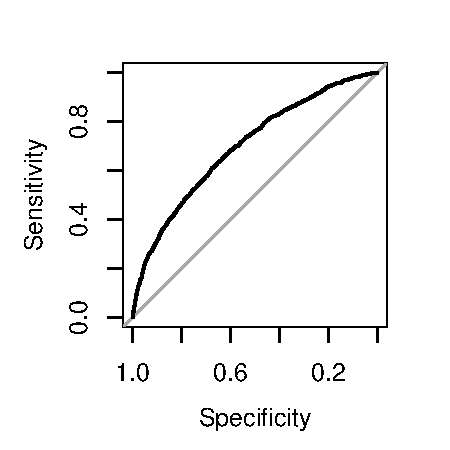
\includegraphics[width=\maxwidth]{figures/knitr-roccurvelogistic-1} 

}



\end{knitrout}
\end{frame}
%%%%%%%%%%%%%%%%%%%%%%%%%%%%%%%%%%%%%%%%%%%%%%%%%%%%%%%%%%%%%%%%%%%%%%%%%


%%%%%%%%%%%%%%%%%%%%%%%%%%%%%%%%%%%%%%%%%%%%%%%%%%%%%%%%%%
\begin{frame}[fragile]{Choice of Decision Rule depends on cost }

\begin{itemize}

\item The aim of this exercise was to highlight that choice of decision criterion, i.e. cutoff $\bar{c}$ need not be dictated by the MAP decision rule that guarantees, on average, best prediction performance.

\item The question really is, what the associated costs are for having many tue positives or true negatives.

\item Optimal choice of $\bar{c}$ would take into account the potentially different costs and may give solutions that are far away from 1/2.

\end{itemize}

\end{frame}
%%%%%%%%%%%%%%%%%%%%%%%%%%%%%%%%%%%%%%%%%%%%%%%%%%%%%%%%%%%%%%%%%%%%%%%%%




%%%%%%%%%%%%%%%%%%%%%%%%%%%%%%%%%%%%%%%%%%%%%%%%%%%%%%%%%%
\begin{frame}[fragile]{Model Selection Approaches}

\begin{itemize}

\item In most machine learning applications, we are worried about overfitting.

\item Overfitting can result from incorporating information contained in features that may explain - by chance - some of the variation in the training set, but perform poorly in the validation set.

\item Shrinkage methods like Lasso can be used to remove features $X$ that do not have a lot of information content in the validation sample

\item Lasso for logistic regression would maximize Log Likelihood minus a penality: 

$$\sum_{i=1}^{n}{y_i \log(p(x_i'\beta)) + (1-y_i) \log((1-p(x_i'\beta)))} -  \lambda \sum_{j=1}^{p} |\beta_j|$$


\end{itemize}

\end{frame}
%%%%%%%%%%%%%%%%%%%%%%%%%%%%%%%%%%%%%%%%%%%%%%%%%%%%%%%%%%%%%%%%%%%%%%%%%


%%%%%%%%%%%%%%%%%%%%%%%%%%%%%%%%%%%%%%%%%%%%%%%%%%%%%%%%%%
\begin{frame}[fragile]{An Example: Spam Data}

\begin{itemize}

\item Most spam detection models use a combination of numeric features derived from the data as well as indicator and counts of word features.

\item Numeric features are measures like the number or share of all caps words, length of uninterruted punctuations, sentence length,... you name it.

\item Dummy variable or count variables of word feature counts.

\item This exercise illustrates estimating logistic regression and performing Lasso to remove the feature space.

\end{itemize}

\end{frame}
%%%%%%%%%%%%%%%%%%%%%%%%%%%%%%%%%%%%%%%%%%%%%%%%%%%%%%%%%%%%%%%%%%%%%%%%%



%%%%%%%%%%%%%%%%%%%%%%%%%%%%%%%%%%%%%%%%%%%%%%%%%%%%%%%%%%
\begin{frame}[fragile]{An Example: Spam Data}

\begin{knitrout}\tiny
\definecolor{shadecolor}{rgb}{0.969, 0.969, 0.969}\color{fgcolor}\begin{kframe}
\begin{alltt}
\hlstd{email} \hlkwb{<-} \hlkwd{read.csv}\hlstd{(}\hlstr{"R/spam.csv"}\hlstd{)}

\hlstd{email}\hlopt{$}\hlstd{spam} \hlkwb{<-} \hlkwd{factor}\hlstd{(email}\hlopt{$}\hlstd{spam,}\hlkwc{levels}\hlstd{=}\hlkwd{c}\hlstd{(}\hlnum{0}\hlstd{,}\hlnum{1}\hlstd{),}\hlkwc{labels}\hlstd{=}\hlkwd{c}\hlstd{(}\hlstr{"important"}\hlstd{,}\hlstr{"spam"}\hlstd{))}

\hlcom{#features}
\hlkwd{names}\hlstd{(email)}
\end{alltt}
\begin{verbatim}
##  [1] "word_freq_make"             "word_freq_address"         
##  [3] "word_freq_all"              "word_freq_3d"              
##  [5] "word_freq_our"              "word_freq_over"            
##  [7] "word_freq_remove"           "word_freq_internet"        
##  [9] "word_freq_order"            "word_freq_mail"            
## [11] "word_freq_receive"          "word_freq_will"            
## [13] "word_freq_people"           "word_freq_report"          
## [15] "word_freq_addresses"        "word_freq_free"            
## [17] "word_freq_business"         "word_freq_email"           
## [19] "word_freq_you"              "word_freq_credit"          
## [21] "word_freq_your"             "word_freq_font"            
## [23] "word_freq_000"              "word_freq_money"           
## [25] "word_freq_hp"               "word_freq_hpl"             
## [27] "word_freq_george"           "word_freq_650"             
## [29] "word_freq_lab"              "word_freq_labs"            
## [31] "word_freq_telnet"           "word_freq_857"             
## [33] "word_freq_data"             "word_freq_415"             
## [35] "word_freq_85"               "word_freq_technology"      
## [37] "word_freq_1999"             "word_freq_parts"           
## [39] "word_freq_pm"               "word_freq_direct"          
## [41] "word_freq_cs"               "word_freq_meeting"         
## [43] "word_freq_original"         "word_freq_project"         
## [45] "word_freq_re"               "word_freq_edu"             
## [47] "word_freq_table"            "word_freq_conference"      
## [49] "char_freq_semicolon"        "char_freq_leftbrac"        
## [51] "char_freq_leftsquarebrac"   "char_freq_exclaim"         
## [53] "char_freq_dollar"           "char_freq_pound"           
## [55] "capital_run_length_average" "capital_run_length_longest"
## [57] "capital_run_length_total"   "spam"
\end{verbatim}
\begin{alltt}
\hlcom{## fit the full model}
\hlstd{spammy} \hlkwb{<-} \hlkwd{glm}\hlstd{(spam} \hlopt{~} \hlstd{.,} \hlkwc{data}\hlstd{=email,} \hlkwc{family}\hlstd{=}\hlstr{'binomial'}\hlstd{)}

\hlkwd{table}\hlstd{(email}\hlopt{$}\hlstd{spam, email}\hlopt{$}\hlstd{word_freq_money}\hlopt{>}\hlnum{0}\hlstd{)}
\end{alltt}
\begin{verbatim}
##            
##             FALSE TRUE
##   important  2734   54
##   spam       1132  681
\end{verbatim}
\begin{alltt}
\hlkwd{plot}\hlstd{(spammy}\hlopt{$}\hlstd{fit}\hlopt{~}\hlstd{email}\hlopt{$}\hlstd{spam,}
        \hlkwc{xlab}\hlstd{=}\hlstr{""}\hlstd{,} \hlkwc{ylab}\hlstd{=}\hlkwd{c}\hlstd{(}\hlstr{"fitted probability of spam"}\hlstd{),}
        \hlkwc{col}\hlstd{=}\hlkwd{c}\hlstd{(}\hlstr{"navy"}\hlstd{,}\hlstr{"red"}\hlstd{))}
\end{alltt}
\end{kframe}

{\centering \includegraphics[width=\maxwidth]{figures/knitr-spammy1-1} 

}



\end{knitrout}

\end{frame}
%%%%%%%%%%%%%%%%%%%%%%%%%%%%%%%%%%%%%%%%%%%%%%%%%%%%%%%%%%%%%%%%%%%%%%%%%


%%%%%%%%%%%%%%%%%%%%%%%%%%%%%%%%%%%%%%%%%%%%%%%%%%%%%%%%%%
\begin{frame}[fragile]{An Example: Validation Set}
\begin{knitrout}\tiny
\definecolor{shadecolor}{rgb}{0.969, 0.969, 0.969}\color{fgcolor}\begin{kframe}
\begin{alltt}
\hlstd{leaveout} \hlkwb{<-} \hlkwd{sample}\hlstd{(}\hlnum{1}\hlopt{:}\hlkwd{nrow}\hlstd{(email),} \hlnum{1000}\hlstd{)} \hlcom{## sample 1000 random indices}
\hlcom{# train the model WITHOUT these observations (-index removes those obs)}
\hlstd{spamtrain} \hlkwb{<-} \hlkwd{glm}\hlstd{(spam} \hlopt{~} \hlstd{.,} \hlkwc{data}\hlstd{=email[}\hlopt{-}\hlstd{leaveout,],} \hlkwc{family}\hlstd{=}\hlstr{'binomial'}\hlstd{)}
\hlcom{# get the predicted probability of spam on the left out data}
\hlstd{pspam} \hlkwb{<-} \hlkwd{predict}\hlstd{(spamtrain,} \hlkwc{newdata}\hlstd{=email[leaveout,],} \hlkwc{type}\hlstd{=}\hlstr{"response"}\hlstd{)}
\hlcom{# plot the OOS fit}
\hlkwd{plot}\hlstd{(pspam} \hlopt{~} \hlstd{email}\hlopt{$}\hlstd{spam[leaveout],}
        \hlkwc{xlab}\hlstd{=}\hlstr{""}\hlstd{,} \hlkwc{ylab}\hlstd{=}\hlkwd{c}\hlstd{(}\hlstr{"predicted probability of spam"}\hlstd{),}
        \hlkwc{col}\hlstd{=}\hlkwd{c}\hlstd{(}\hlstr{"navy"}\hlstd{,}\hlstr{"red"}\hlstd{))}
\end{alltt}
\end{kframe}

{\centering \includegraphics[width=2in]{figures/knitr-spammy2-1} 

}



\end{knitrout}

\end{frame}
%%%%%%%%%%%%%%%%%%%%%%%%%%%%%%%%%%%%%%%%%%%%%%%%%%%%%%%%%%%%%%%%%%%%%%%%%



%%%%%%%%%%%%%%%%%%%%%%%%%%%%%%%%%%%%%%%%%%%%%%%%%%%%%%%%%%
\begin{frame}[fragile]{An Example: Regularized Regression}
\begin{knitrout}\tiny
\definecolor{shadecolor}{rgb}{0.969, 0.969, 0.969}\color{fgcolor}\begin{kframe}
\begin{alltt}
\hlstd{x}\hlkwb{<-}\hlkwd{model.matrix}\hlstd{(spam}\hlopt{~}\hlstd{.,} \hlkwc{data}\hlstd{=email)[,}\hlopt{-}\hlnum{1}\hlstd{]}

\hlstd{lasso.mod}\hlkwb{=}\hlkwd{glmnet}\hlstd{(x,} \hlkwd{as.factor}\hlstd{(email}\hlopt{$}\hlstd{spam),}\hlkwc{alpha}\hlstd{=}\hlnum{1}\hlstd{,}\hlkwc{standardize}\hlstd{=}\hlnum{TRUE}\hlstd{,}\hlkwc{family}\hlstd{=}\hlstr{'binomial'}\hlstd{)}

\hlkwd{plot}\hlstd{(lasso.mod,} \hlkwc{xvar}\hlstd{=}\hlstr{"lambda"}\hlstd{)}
\end{alltt}
\end{kframe}

{\centering \includegraphics[width=2in]{figures/knitr-spammy3-1} 

}



\end{knitrout}

\end{frame}
%%%%%%%%%%%%%%%%%%%%%%%%%%%%%%%%%%%%%%%%%%%%%%%%%%%%%%%%%%%%%%%%%%%%%%%%%


%%%%%%%%%%%%%%%%%%%%%%%%%%%%%%%%%%%%%%%%%%%%%%%%%%%%%%%%%%
\begin{frame}[fragile]{An Example: Cross Validation for Parameter Selection}
\begin{knitrout}\tiny
\definecolor{shadecolor}{rgb}{0.969, 0.969, 0.969}\color{fgcolor}\begin{kframe}
\begin{alltt}
\hlstd{cv.glmmod}\hlkwb{<-}\hlkwd{cv.glmnet}\hlstd{(x,}\hlkwc{y}\hlstd{=}\hlkwd{as.factor}\hlstd{(email}\hlopt{$}\hlstd{spam),}\hlkwc{alpha}\hlstd{=}\hlnum{1}\hlstd{,}\hlkwc{standardize}\hlstd{=}\hlnum{TRUE}\hlstd{,}\hlkwc{family}\hlstd{=}\hlstr{"binomial"}\hlstd{)}

 \hlkwd{plot}\hlstd{(cv.glmmod)}


\hlstd{cv.glmmod}\hlopt{$}\hlstd{lambda.min}
\end{alltt}
\begin{verbatim}
## [1] 0.000403
\end{verbatim}
\end{kframe}

{\centering \includegraphics[width=2in]{figures/knitr-spammy4-1} 

}



\end{knitrout}

\end{frame}
%%%%%%%%%%%%%%%%%%%%%%%%%%%%%%%%%%%%%%%%%%%%%%%%%%%%%%%%%%%%%%%%%%%%%%%%%


\section{Working with Text features}

%%%%%%%%%%%%%%%%%%%%%%%%%%%%%%%%%%%%%%%%%%%%%%%%%%%%%%%%%%%%%%%%%%%%%%%%%
\begin{frame}{Working with text features}

\begin{itemize}

\item For short fragments, its most often useful to just dummify features

\item Word counts at the sentence level do not make much sense

\item I will show an example of logistic regression or multionomial logistic regression applied to a case of two categories categorizing short pieces of text.


\end{itemize}

\end{frame}
%%%%%%%%%%%%%%%%%%%%%%%%%%%%%%%%%%%%%%%%%%%%%%%%%%%%%%%%%%



%%%%%%%%%%%%%%%%%%%%%%%%%%%%%%%%%%%%%%%%%%%%%%%%%%%%%%%%%%%%%%%%%%%%%%%%%
\begin{frame}[fragile]{Working with text features}
\begin{knitrout}\tiny
\definecolor{shadecolor}{rgb}{0.969, 0.969, 0.969}\color{fgcolor}\begin{kframe}
\begin{alltt}
\hlkwd{library}\hlstd{(data.table)}
\hlkwd{library}\hlstd{(haven)}
\hlstd{DTA}\hlkwb{<-}\hlkwd{data.table}\hlstd{(}\hlkwd{read_dta}\hlstd{(}\hlkwc{file}\hlstd{=}\hlstr{"/Users/thiemo/Dropbox/Research/Blog/immigration/data/bes_f2f_original_v3.0.dta"}\hlstd{))}
\hlstd{DTA[, .N,} \hlkwc{by}\hlstd{=A1][}\hlkwd{order}\hlstd{(N,}\hlkwc{decreasing}\hlstd{=}\hlnum{TRUE}\hlstd{)][}\hlnum{1}\hlopt{:}\hlnum{10}\hlstd{]}
\end{alltt}
\begin{verbatim}
##               A1   N
##  1:  immigration 227
##  2:              131
##  3:  Immigration  52
##  4:      economy  44
##  5:          NHS  41
##  6: unemployment  40
##  7:    terrorism  24
##  8:  IMMIGRATION  20
##  9:   immigrants  20
## 10:  the economy  18
\end{verbatim}
\begin{alltt}
\hlstd{DTA[}\hlkwd{grep}\hlstd{(}\hlstr{"immi"}\hlstd{,A1,} \hlkwc{ignore.case}\hlstd{=}\hlnum{TRUE}\hlstd{)][}\hlkwd{nchar}\hlstd{(A1)}\hlopt{>}\hlnum{10}\hlstd{][}\hlnum{1}\hlopt{:}\hlnum{3}\hlstd{]}\hlopt{$}\hlstd{A1}
\end{alltt}
\begin{verbatim}
## [1] "Immigration"         "too many immigrants" "Immigration"        
## attr(,"label")
## [1] "A1: Most important issue"
## attr(,"format.stata")
## [1] "%244s"
\end{verbatim}
\end{kframe}
\end{knitrout}
\end{frame}
%%%%%%%%%%%%%%%%%%%%%%%%%%%%%%%%%%%%%%%%%%%%%%%%%%%%%%%%%%


%%%%%%%%%%%%%%%%%%%%%%%%%%%%%%%%%%%%%%%%%%%%%%%%%%%%%%%%%%%%%%%%%%%%%%%%%
\begin{frame}[fragile]{Defining text features for predictive exercise}
\begin{knitrout}\tiny
\definecolor{shadecolor}{rgb}{0.969, 0.969, 0.969}\color{fgcolor}\begin{kframe}
\begin{alltt}
\hlcom{##use document scaling method to define features}
\hlstd{DTA[, leaveeu} \hlkwb{:=} \hlstr{"remain"}\hlstd{]}
\hlstd{DTA[p02}\hlopt{==}\hlnum{1}\hlstd{, leaveeu} \hlkwb{:=} \hlstr{"leave"}\hlstd{]}
\hlstd{DTA[p02}\hlopt{<}\hlnum{0} \hlopt{|}\hlstd{p02}\hlopt{>}\hlnum{2}\hlstd{, leaveeu} \hlkwb{:=} \hlnum{NA} \hlstd{]}
\hlstd{DTA[, leaveeu} \hlkwb{:=} \hlkwd{as.factor}\hlstd{(leaveeu)]}
\hlstd{DTA[, toomanyimmigrants} \hlkwb{:=} \hlkwd{as.numeric}\hlstd{(j05}\hlopt{==}\hlnum{1}\hlstd{)]}
\hlstd{DTA[j05}\hlopt{<}\hlnum{0} \hlopt{|}\hlstd{j05}\hlopt{>}\hlnum{2}\hlstd{, toomanyimmigrants} \hlkwb{:=} \hlnum{NA} \hlstd{]}
\hlstd{DTA}\hlkwb{<-}\hlstd{DTA[}\hlopt{!}\hlkwd{is.na}\hlstd{(leaveeu)} \hlopt{& !}\hlkwd{is.na}\hlstd{(toomanyimmigrants)]}
\hlkwd{table}\hlstd{(DTA[ ,}\hlkwd{list}\hlstd{(toomanyimmigrants, leaveeu)])}
\end{alltt}
\begin{verbatim}
##                  leaveeu
## toomanyimmigrants leave remain
##                 0    60    478
##                 1   872    777
\end{verbatim}
\begin{alltt}
\hlkwd{library}\hlstd{(quanteda)}
\hlstd{C}\hlkwb{<-}\hlkwd{corpus}\hlstd{(DTA}\hlopt{$}\hlstd{A1)}
\hlcom{##defining features that are informative about leaveeu decision using e.g. document scaling method}
\hlkwd{docnames}\hlstd{(C)}\hlkwb{<-}\hlstd{DTA}\hlopt{$}\hlstd{finalserialno}
\hlstd{C.dfm}\hlkwb{<-}\hlkwd{dfm}\hlstd{(C,} \hlkwc{tolower} \hlstd{=} \hlnum{TRUE}\hlstd{,} \hlkwc{stem} \hlstd{=} \hlnum{TRUE}\hlstd{,} \hlkwc{removeNumbers}\hlstd{=}\hlnum{TRUE}\hlstd{,}\hlkwc{removePunct}\hlstd{=}\hlnum{TRUE}\hlstd{,} \hlkwc{remove} \hlstd{=} \hlkwd{stopwords}\hlstd{(}\hlstr{"english"}\hlstd{))}
\end{alltt}
\end{kframe}
\end{knitrout}
\end{frame}
%%%%%%%%%%%%%%%%%%%%%%%%%%%%%%%%%%%%%%%%%%%%%%%%%%%%%%%%%%


%%%%%%%%%%%%%%%%%%%%%%%%%%%%%%%%%%%%%%%%%%%%%%%%%%%%%%%%%%%%%%%%%%%%%%%%%
\begin{frame}[fragile]{Single most important issue facing the UK in 2015}
\begin{knitrout}\tiny
\definecolor{shadecolor}{rgb}{0.969, 0.969, 0.969}\color{fgcolor}\begin{kframe}
\begin{alltt}
\hlkwd{plot}\hlstd{(C.dfm)}
\end{alltt}
\end{kframe}

{\centering \includegraphics[width=3in]{figures/knitr-brexitexample3-1} 

}



\end{knitrout}
\end{frame}
%%%%%%%%%%%%%%%%%%%%%%%%%%%%%%%%%%%%%%%%%%%%%%%%%%%%%%%%%%


%%%%%%%%%%%%%%%%%%%%%%%%%%%%%%%%%%%%%%%%%%%%%%%%%%%%%%%%%%%%%%%%%%%%%%%%%
\begin{frame}[fragile]{Bayes scoring to identify relevant features}
\begin{knitrout}\tiny
\definecolor{shadecolor}{rgb}{0.969, 0.969, 0.969}\color{fgcolor}\begin{kframe}
\begin{alltt}
\hlcom{##use document scaling method to define features}

\hlcom{##using Bayes scores to identify particular word features associated with Brexit}
\hlkwd{summary}\hlstd{(DTA}\hlopt{$}\hlstd{leaveeu)}
\end{alltt}
\begin{verbatim}
##  leave remain 
##    932   1255
\end{verbatim}
\begin{alltt}
\hlstd{ws2} \hlkwb{<-} \hlkwd{textmodel}\hlstd{(C.dfm,} \hlkwd{as.numeric}\hlstd{(DTA}\hlopt{$}\hlstd{leaveeu),} \hlkwc{model}\hlstd{=}\hlstr{"NB"}\hlstd{,} \hlkwc{smooth}\hlstd{=}\hlnum{0}\hlstd{)}

\hlcom{#Words associated with LEAVE }
\hlstd{scores}\hlkwb{<-}\hlkwd{sort}\hlstd{(}\hlkwd{log}\hlstd{(ws2}\hlopt{$}\hlstd{PwGc[}\hlnum{1}\hlstd{,]}\hlopt{/}\hlstd{ws2}\hlopt{$}\hlstd{PwGc[}\hlnum{2}\hlstd{,]),}\hlkwc{decreasing}\hlstd{=}\hlnum{FALSE}\hlstd{)}
\hlstd{scores}\hlkwb{<-}\hlstd{scores[}\hlkwd{names}\hlstd{(}\hlkwd{topfeatures}\hlstd{(C.dfm,} \hlkwc{n}\hlstd{=}\hlnum{250}\hlstd{))]}
\hlstd{scores}\hlkwb{<-}\hlstd{scores[}\hlopt{!}\hlkwd{is.infinite}\hlstd{(scores)]}
\hlstd{scores}\hlkwb{<-}\hlkwd{sort}\hlstd{(scores)}

\hlkwd{head}\hlstd{(scores)}
\end{alltt}
\begin{verbatim}
##    societi      young      littl    minimum manufactur       deal 
##      -1.95      -1.73      -1.73      -1.73      -1.73      -1.60
\end{verbatim}
\begin{alltt}
\hlstd{features}\hlkwb{<-}\hlkwd{names}\hlstd{(}\hlkwd{c}\hlstd{(}\hlkwd{head}\hlstd{(scores,}\hlnum{100}\hlstd{),}\hlkwd{tail}\hlstd{(scores,} \hlnum{100}\hlstd{)))}
\hlstd{features}\hlkwb{<-}\hlstd{features[}\hlkwd{nchar}\hlstd{(features)}\hlopt{>}\hlnum{3}\hlstd{]}
\end{alltt}
\end{kframe}
\end{knitrout}
\end{frame}
%%%%%%%%%%%%%%%%%%%%%%%%%%%%%%%%%%%%%%%%%%%%%%%%%%%%%%%%%%



%%%%%%%%%%%%%%%%%%%%%%%%%%%%%%%%%%%%%%%%%%%%%%%%%%%%%%%%%%%%%%%%%%%%%%%%%
\begin{frame}[fragile]{Bayes scoring to identify relevant features}
\begin{knitrout}\tiny
\definecolor{shadecolor}{rgb}{0.969, 0.969, 0.969}\color{fgcolor}\begin{kframe}
\begin{alltt}
\hlcom{##remove features not in the leave/ remain list}
\hlkwd{dim}\hlstd{(C.dfm)}
\end{alltt}
\begin{verbatim}
## [1] 2187 1653
\end{verbatim}
\begin{alltt}
\hlstd{C.subdfm}\hlkwb{<-}\hlkwd{dfm_select}\hlstd{(C.dfm,} \hlkwc{features}\hlstd{=features ,} \hlkwc{selection}\hlstd{=}\hlstr{"keep"}\hlstd{)}

\hlkwd{dim}\hlstd{(C.subdfm)}
\end{alltt}
\begin{verbatim}
## [1] 2187  171
\end{verbatim}
\begin{alltt}
\hlcom{##convert DFM into a simple matrix }
\hlstd{MAT}\hlkwb{<-}\hlkwd{data.frame}\hlstd{(}\hlstr{"leaveeu"}\hlstd{=DTA}\hlopt{$}\hlstd{leaveeu, C.subdfm)}
\hlstd{leaveout} \hlkwb{<-} \hlkwd{sample}\hlstd{(}\hlnum{1}\hlopt{:}\hlkwd{nrow}\hlstd{(MAT),} \hlnum{200}\hlstd{)} \hlcom{## sample 500 random indices}
\hlcom{# train the model WITHOUT these observations (-index removes those obs)}
\hlstd{trained} \hlkwb{<-} \hlkwd{glm}\hlstd{(leaveeu} \hlopt{~} \hlstd{.,} \hlkwc{data}\hlstd{=MAT[}\hlopt{-}\hlstd{leaveout,],} \hlkwd{binomial}\hlstd{(}\hlkwc{link}\hlstd{=logit))}
\hlcom{# get the predicted probability of spam on the left out data}
\hlstd{glm.probs} \hlkwb{<-} \hlkwd{predict}\hlstd{(trained,} \hlkwc{newdata}\hlstd{=MAT[leaveout,],} \hlkwc{type}\hlstd{=}\hlstr{"response"}\hlstd{)}
\hlcom{# plot the OOS fit}

\hlstd{glm.pred}\hlkwb{=}\hlkwd{rep}\hlstd{(}\hlstr{"remain"}\hlstd{,}\hlkwd{length}\hlstd{(glm.probs))}
\hlstd{glm.pred[glm.probs}\hlopt{>}\hlnum{0.5}\hlstd{]}\hlkwb{=}\hlstr{"leave"}

\hlkwd{table}\hlstd{(glm.pred,MAT[leaveout,]}\hlopt{$}\hlstd{leaveeu)}
\end{alltt}
\begin{verbatim}
##         
## glm.pred leave remain
##   leave     42     95
##   remain    38     25
\end{verbatim}
\end{kframe}
\end{knitrout}
\end{frame}
%%%%%%%%%%%%%%%%%%%%%%%%%%%%%%%%%%%%%%%%%%%%%%%%%%%%%%%%%%


%%%%%%%%%%%%%%%%%%%%%%%%%%%%%%%%%%%%%%%%%%%%%%%%%%%%%%%%%%
\begin{frame}[fragile]{Simple MaxEnt Classification in RTextTools}
\begin{knitrout}\tiny
\definecolor{shadecolor}{rgb}{0.969, 0.969, 0.969}\color{fgcolor}\begin{kframe}
\begin{alltt}
\hlkwd{set.seed}\hlstd{(}\hlnum{2016}\hlstd{)}
\hlstd{TRAINING}\hlkwb{<-}\hlkwd{data.table}\hlstd{(}\hlkwd{read.csv}\hlstd{(}\hlkwc{file}\hlstd{=}\hlstr{"/Users/thiemo/Dropbox/Research/Matteo and Thiemo/senna/classification-tree.csv"}\hlstd{))}

\hlstd{PERSON}\hlkwb{<-}\hlstd{TRAINING[objecttype}\hlopt{==}\hlstr{"person"} \hlopt{&} \hlstd{label1}\hlopt{!=}\hlstr{""}\hlstd{]}
\hlstd{PERSON}\hlopt{$}\hlstd{label1} \hlkwb{<-} \hlkwd{factor}\hlstd{(PERSON}\hlopt{$}\hlstd{label1)}
\hlstd{PERSON}\hlopt{$}\hlstd{label1num} \hlkwb{<-} \hlkwd{as.numeric}\hlstd{(}\hlkwd{factor}\hlstd{(PERSON}\hlopt{$}\hlstd{label1))}

\hlkwd{head}\hlstd{(PERSON[label1} \hlopt{==}\hlstr{"civilian"}\hlstd{,}\hlkwd{paste}\hlstd{(verb,objectcleanpp,}\hlkwc{sep}\hlstd{=}\hlstr{" "}\hlstd{)])}
\end{alltt}
\begin{verbatim}
## [1] "abducted civilians village morian"                                            
## [2] "killed civilians"                                                             
## [3] "kidnapped civilian dingdongpara"                                              
## [4] "killed civilian who had reportedly functioned counter insurgent few years ago"
## [5] "killed civilian"                                                              
## [6] "abducted civilians"
\end{verbatim}
\end{kframe}
\end{knitrout}
\end{frame}
%%%%%%%%%%%%%%%%%%%%%%%%%%%%%%%%%%%%%%%%%%%%%%%%%%%%%%%%%%%%%%%%%%%%%%%%%



%%%%%%%%%%%%%%%%%%%%%%%%%%%%%%%%%%%%%%%%%%%%%%%%%%%%%%%%%%
\begin{frame}[fragile]{An Example on how to do simple MaxEnt Classification}
\begin{knitrout}\tiny
\definecolor{shadecolor}{rgb}{0.969, 0.969, 0.969}\color{fgcolor}\begin{kframe}
\begin{alltt}
\hlkwd{head}\hlstd{(PERSON[label1} \hlopt{==}\hlstr{"terrorist"}\hlstd{,}\hlkwd{paste}\hlstd{(verb,objectcleanpp,}\hlkwc{sep}\hlstd{=}\hlstr{" "}\hlstd{)])}
\end{alltt}
\begin{verbatim}
## [1] "killed maoist cpi aoist cadre"                      
## [2] "raided maoist hideout village forest area abuj mad" 
## [3] "surrendered maoists"                                
## [4] "killed terrorists united liberation front asom ulfa"
## [5] "injuring least militants"                           
## [6] "arrested cpi aoist cadres village"
\end{verbatim}
\end{kframe}
\end{knitrout}
\end{frame}
%%%%%%%%%%%%%%%%%%%%%%%%%%%%%%%%%%%%%%%%%%%%%%%%%%%%%%%%%%%%%%%%%%%%%%%%%


%%%%%%%%%%%%%%%%%%%%%%%%%%%%%%%%%%%%%%%%%%%%%%%%%%%%%%%%%%
\begin{frame}[fragile]{An Example on how to do simple MaxEnt Classification}
\begin{knitrout}\tiny
\definecolor{shadecolor}{rgb}{0.969, 0.969, 0.969}\color{fgcolor}\begin{kframe}
\begin{alltt}
\hlkwd{library}\hlstd{(tm)}
\hlkwd{library}\hlstd{(RTextTools)}
\hlkwd{set.seed}\hlstd{(}\hlnum{30012017}\hlstd{)}
\hlcom{#a validation set}
\hlstd{valid}\hlkwb{<-}\hlkwd{sample}\hlstd{(}\hlnum{1}\hlopt{:}\hlkwd{nrow}\hlstd{(PERSON),} \hlnum{500}\hlstd{)}
\hlstd{PERSON}\hlopt{$}\hlstd{validation}\hlkwb{<-} \hlnum{0}
\hlstd{PERSON[valid]}\hlopt{$}\hlstd{validation}\hlkwb{<-}\hlnum{1}
\hlstd{PERSON}\hlkwb{<-}\hlstd{PERSON[}\hlkwd{order}\hlstd{(validation)]}
\hlstd{DOC}\hlkwb{<-}\hlkwd{create_matrix}\hlstd{(}\hlkwd{c}\hlstd{(PERSON[,}\hlkwd{paste}\hlstd{(objectcleanpp,}\hlkwc{sep}\hlstd{=}\hlstr{" "}\hlstd{)]),}\hlkwc{language}\hlstd{=}\hlstr{"english"}\hlstd{,}
                   \hlkwc{removeNumbers}\hlstd{=}\hlnum{TRUE}\hlstd{,}\hlkwc{stemWords}\hlstd{=}\hlnum{TRUE}\hlstd{,}\hlkwc{removePunctuation}\hlstd{=}\hlnum{TRUE}\hlstd{,}\hlkwc{removeSparseTerms}\hlstd{=}\hlnum{0.9999}\hlstd{)}
\hlstd{DOCCONT}\hlkwb{<-}\hlkwd{create_container}\hlstd{(DOC,PERSON}\hlopt{$}\hlstd{label1num,} \hlkwc{trainSize}\hlstd{=}\hlnum{1}\hlopt{:}\hlnum{1200}\hlstd{,}
                          \hlkwc{testSize}\hlstd{=}\hlnum{1201}\hlopt{:}\hlkwd{nrow}\hlstd{(PERSON),} \hlkwc{virgin}\hlstd{=}\hlnum{TRUE}\hlstd{)}
\hlstd{MOD} \hlkwb{<-} \hlkwd{train_models}\hlstd{(DOCCONT,} \hlkwc{algorithms}\hlstd{=}\hlkwd{c}\hlstd{(}\hlstr{"MAXENT"}\hlstd{))}
\hlstd{RES} \hlkwb{<-} \hlkwd{classify_models}\hlstd{(DOCCONT, MOD)}
\hlstd{analytics} \hlkwb{<-} \hlkwd{create_analytics}\hlstd{(DOCCONT, RES)}
\hlstd{res}\hlkwb{<-}\hlkwd{data.table}\hlstd{(analytics}\hlopt{@}\hlkwc{document_summary}\hlstd{)}
\hlstd{VALID}\hlkwb{<-}\hlkwd{cbind}\hlstd{(PERSON[validation}\hlopt{==}\hlnum{1}\hlstd{],res)}

\hlcom{#confusion matrix}
\hlkwd{table}\hlstd{(VALID}\hlopt{$}\hlstd{label1,}\hlkwd{factor}\hlstd{(VALID}\hlopt{$}\hlstd{MAXENTROPY_LABEL,} \hlkwc{labels}\hlstd{=}\hlkwd{levels}\hlstd{(VALID}\hlopt{$}\hlstd{label1)))}
\end{alltt}
\begin{verbatim}
##            
##             civilian security terrorist
##   civilian        96        7        13
##   security         5       93         6
##   terrorist       14        5       261
\end{verbatim}
\begin{alltt}
\hlkwd{sum}\hlstd{(}\hlkwd{diag}\hlstd{(}\hlnum{3}\hlstd{)} \hlopt{*}\hlkwd{table}\hlstd{(VALID}\hlopt{$}\hlstd{MAXENTROPY_LABEL,VALID}\hlopt{$}\hlstd{label1))}\hlopt{/}\hlnum{500}
\end{alltt}
\begin{verbatim}
## [1] 0.9
\end{verbatim}
\end{kframe}
\end{knitrout}
\end{frame}
%%%%%%%%%%%%%%%%%%%%%%%%%%%%%%%%%%%%%%%%%%%%%%%%%%%%%%%%%%%%%%%%%%%%%%%%%



\end{document}

